\section{Entwicklung \& Verwendung des Compilers}

    \subsection{Verwendung des Compilers}
        Der Compiler wird in der Kommandozeile ausgeführt.
        Um den Programmcode zu kompilieren, wird der Pfad der Hauptdatei (also die Datei, 
        in der sich die \texttt{main} Funktion befindet) als Argument übergeben. Sofern eine lokale Installation 
        des Clang Compilers vorhanden ist, verwendet mein Compiler diese um die LLVM IR in eine ausführbare Datei umzuwandeln.
        Die ausführbare Datei wird im cwd (current working directory, also in dem Pfad in dem der Compiler ausgeführt wird) erstellt.

        \noindent Es gibt folgende optionale Argumente:
        \begin{itemize}
            \item \texttt{-e, --emit-llvm}: Der Compiler gibt die LLVM-IR aus.
            \item \texttt{-o, --output}: Der Pfad der ausführbaren Datei (standardmäßig \texttt{./out.exe}).
            \item \texttt{-h, --help}: Gibt die Hilfe aus.
            \item \texttt{-v, --version}: Gibt die Version des Compilers aus.
        \end{itemize}

    \subsection{Arten von Programmiersprachen}
        \subsubsection{Interpreter}
            \emph{Interpreter}\footnote{Interpreter: \url{https://de.wikipedia.org/wiki/Interpreter}} sind Programme, die interpretierte Programmiersprachen meist Zeile für Zeile ausführen. Das hat den Vorteil, dass interpretierte Sprachen leichter zu debuggen
            sind und auf allen Plattformen funktionieren, auf denen der Interpreter verfügbar ist. Bekannte Beispiele sind Python und JavaScript.
            Ein Nachteil ist, dass interpretierte Sprachen einen Interpreter benötigen, um ausgeführt zu werden und meist um ein Vielfaches langsamer sind als kompilierte Sprachen.    

        \subsubsection{Compiler}
            \emph{Compiler}\footnote{Compiler: \url{https://de.wikipedia.org/wiki/Compiler}} übersetzen den Quellcode eines Programms in eine Form, die direkt von Computern ausgeführt werden kann.
            Bekannte Beispiele sind C, C++, Rust und Go.
            Der Vorteil von kompilierten Sprachen ist, dass kein externes Programm benötigt wird, um Programme auszuführen.
        \subsubsection{Transpiler}
            \emph{Transpiler}\footnote{Transpiler: \url{https://en.wikipedia.org/wiki/Source-to-source_compiler}} oder Source-to-Source (S2S) Compiler übersetzen eine Programmiersprache in eine andere. Dabei sind beide Sprachen in der Regel von Menschen lesbar.
            Bekannte Beispiele sind TypeScript und V-lang.

    \subsection{LLVM IR}
        Bei \emph{LLVM IR}\footnote{LLVM IR: \url{https://llvm.org/docs/LangRef.html}} (LLVM Intermediate Representation) handelt es sich um eine plattformunabhängige Zwischensprache, die sehr wenig Abstraktion bietet und daher im Umfang und in den Funktionen recht simpel ist.
        Diese Zwischensprache kann von dem LLC (LLVM static compiler) oder einem Compiler, der diesen verwendet (z.B. Clang), in plattformabhängige Maschinensprache übersetzt werden.
        LLVM IR wird von Compilern wie Clang, Clang++ oder Rustc verwendet.
    \subsection{Compilerarchitektur}
        Nun werde ich auf die Architektur meines Compilers eingehen.
        Zunächst habe ich mich für eine kompilierte Sprache entschieden, da ich keine zur Ausführung der Programme keine 
        externe Laufzeitumgebung haben wollte.

        \subsubsection{Frontend}

            \begin{center}
                \textbf{Lexer\footnote{Codeverweis Tokens: \texttt{src/lexer/tokens.rs}, Lexer: \texttt{src/lexer/lexer_main.rs}}}
            \end{center}

            Das Compiler Frontend ist der Teil eines Compilers, der den Quellcode eines Programms liest und in 
            eine Datenstruktur übersetzt (meist ein abstrakter Syntaxbaum (AST)). 

            Der Quellcode wird zu Beginn von einem Lexer in eine Liste von Tokens übersetzt.
            Dabei wird Zeichen für Zeichen vorgegangen.

            Ein Hello World Programm wird folgendermaßen in Tokens übersetzt:
            \newpage
            \begin{lstlisting}
                use "std/io.mx"

                def main() -> int {
                    println("Hello, World!");
                    return 0;
                }
            \end{lstlisting}

            \begin{center}
                \begin{tabular}{|c|c|}
                    \hline
                    Quellcode & Token \\
                    \hline
                    use & Keyword::Use \\
                    ''std/io.mx'' & String ''std/io.mx'' \\
                    def & Keyword::Def \\
                    main & Identifier "main" \\
                    ( & Punctuation::OpenParen \\
                    ) & Punctuation::CloseParen \\
                    -\textgreater & Punctuation::ThinArrow \\
                    int & Identifier "int" \\
                    \{ & Punctuation::OpenBrace \\
                    println & Identifier "println" \\
                    ( & Punctuation::OpenParen \\
                    "Hello, World!" & String "Hello, World!" \\
                    ) & Punctuation::CloseParen \\
                    ; & Punctuation::Semicolon \\
                    return & Keyword::Return \\
                    0 & Literal::Integer 0 \\
                    ; & Punctuation::Semicolon \\
                    \} & Punctuation::CloseBrace \\
                    \hline
 
                \end{tabular}
            \end{center}

        Während der Tokenisierung werden für jedes Token auch noch die Positionen im Quellcode 
        mitgespeichert, um später bei Fehlermeldungen die Position des Fehlers
        anzeigen zu können.

        \begin{center}
            \textbf{Parser und AST\footnote{Codeverweis Parser: \texttt{src/parser/parser_main.rs}, AST: \texttt{src/parser/ast.rs}}}
        \end{center}

        Anschließend wird ein \texttt{Parser} Objekt erstellt. Dieser geht nun die Liste von Tokens
        der Reihe nach durch und erstellt einen abstrakten Syntaxbaum (AST). Der Parser hat einen Zustand,
        der sich bei der Erstellung des Syntaxbaumes verändert. Der Parser speichert z.B. 
        definierte Funktionen und Klassen in separaten Listen. Wenn nun z.B. eine Klasse \texttt{Foo} definiert wird,
        erstellt der Parser intern eine Klassenstruktur und speichert diese ab.
        Wenn nun im Programm ein \texttt{Token::Identifier "Foo"} gefunden wird, kann der Parser auf
        die gespeicherte Klasse \texttt{Foo} zugreifen.
        Selbes gilt auch für Funktionen und Variablen.

        Nachdem ein Syntaxbaum erstellt wurde, sieht er vereinfacht so aus:

        \begin{center}

            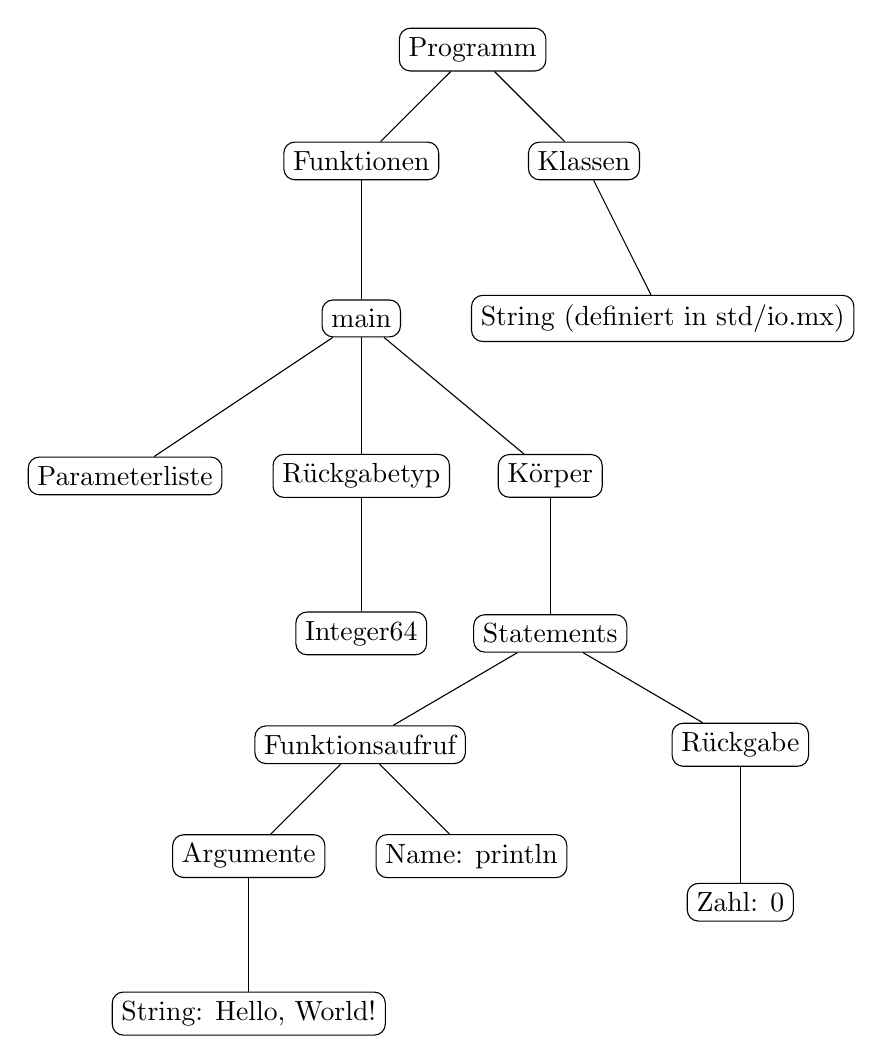
\begin{tikzpicture}[
                node distance=2cm,
                auto,
                block/.style={
                    rectangle,
                    draw,
                    align=center,
                    rounded corners
                },
                line/.style={
                    draw,
                }]
            
                \node [block] (programm) {Programm};
                \node [block, below left of=programm] (funktionen) {Funktionen};
                \node [block, below right of=programm] (klassen) {Klassen};

                \node [block, below of=klassen, xshift=1cm] (string_class) {String (definiert in std/io.mx)};
            
                \node [block, below of=funktionen] (main) {main};

                \node [block, below of=main, xshift=-3cm] (parameterliste) {Parameterliste};
                \node [block, below of=main] (rueckgabetyp) {Rückgabetyp};
                \node [block, below of=main, xshift=2.4cm] (koerper) {Körper};

                \node [block, below of=rueckgabetyp] (int) {Integer64};
                \node [block, below of=koerper] (statements) {Statements};

                \node [block, below left of=statements, xshift=-1cm] (funktionsaufruf) {Funktionsaufruf};
                \node [block, below right of=funktionsaufruf] (funktionsname) {Name: println};

                \node [block, below left of=funktionsaufruf] (argumente) {Argumente};
                \node [block, below of=argumente] (string) {String: Hello, World!};

                \node [block, below right of=statements, xshift=1cm] (return) {Rückgabe};
                \node [block, below of=return] (literal_0) {Zahl: 0};

                \draw [line] (programm) -- (funktionen);
                \draw [line] (programm) -- (klassen);

                \draw [line] (klassen) -- (string_class);
                
                \draw [line] (funktionen) -- (main);
                \draw [line] (main) -- (parameterliste);
                \draw [line] (main) -- (rueckgabetyp);
                \draw [line] (main) -- (koerper);

                \draw [line] (rueckgabetyp) -- (int);
                \draw [line] (koerper) -- (statements);

                \draw [line] (statements) -- (funktionsaufruf);
                \draw [line] (funktionsaufruf) -- (funktionsname);

                \draw [line] (funktionsaufruf) -- (argumente);
                \draw [line] (argumente) -- (string);

                \draw [line] (statements) -- (return);
                \draw [line] (return) -- (literal_0);

            \end{tikzpicture}

        \end{center}

        % \vspace{1cm}
        \newpage
        Die \texttt{String} Klasse wird im Parser folgendermaßen gespeichert:

        \begin{center}
            \begin{tabular}{|c|c|}
                \hline
                Anzeigename & String \\
                \hline
                Name & String \\
                \hline
                Felder & 
                \begin{tabular}{c|c}
                    Name & Typ \\
                    \hline
                    Datenzeiger & *int8 \\
                    Länge & int64 \\
                    Kapazität & int64 \\
                \end{tabular} \\
                \hline

                Subtypen & - \\
                \hline
                Generics & - \\
                \hline
                Subtyp von & - \\
                \hline

            \end{tabular}
        \end{center}

        % \newpage

        \begin{center}
            \textbf{Generics\footnote{Codeverweis: \texttt{src/parser/utils.rs}}} 
        \end{center}

        Da meine Sprache auch Generics in Funktionen und Klassen unterstützt, werde ich erklären wie diese in meinem
        Compiler implementiert sind.

        % Wie in der oberen Tabelle zu sehen ist, hat jede Klasse die Felder \texttt{Generics}, \texttt{Subtypen} und \texttt{Subtyp von}.
        % Mein Compiler verwendet, um dynamische Unterklassen zu erstellen, z.B. wenn es eine generische Klasse 
        % \texttt{List<T>} gibt, und eine Klasse \texttt{List} mit einem spezifischen Typen \texttt{int} erstellt wird, wird eine neue Klasse 
        % \texttt{ListInt} erstellt, die alle Datentypen \texttt{T} in Feldern und Methoden durch \texttt{int} ersetzt.

        Wie in der oberen Tabelle zu sehen ist, besitzt jede Klasse die Felder \texttt{Generics}, \texttt{Subtypen} und \texttt{Subtyp von}.
        Diese verwendet mein Compiler, um dynamische Unterklassen zu erstellen. Dies passiert, wenn eine generische Klasse
        mit einem spezifischen Typen instanziiert wird. Wenn es z.B. eine generische Klasse \texttt{List<T>} gibt,
        und ein Datenobjekt erstellt wird, bei dem \texttt{T} durch \texttt{int} ersetzt wird (\texttt{List<int>}), wird eine neue Klasse+
        \texttt{ListInt} erstellt, die alle Vorkommen von \texttt{T} in Feldern und Methoden durch \texttt{int} ersetzt.

        Das folgende Beispiel veranschaulicht diese dynamische Typerstellung (im echten Compiler wird dies während der 
        Erstellung des Syntaxbaums gemacht, Code in meiner Sprache wird für Generics also nicht erzeugt):
        % \begin{adjustwidth}{-1.7cm}{1cm}

        \begin{center}
            \begin{tabular}{c|c}
                Quellcode & "Generierter Code" \\
                \hline
                \begin{minipage}{0.45\textwidth}
                    \begin{lstlisting}
class Foo<T> {
    data: T,
}

class Bar {
    data: int,
}
        
def main() -> int {
    let bar = Bar { 
        data: 5 
    };
    return bar.data;
}
            \end{lstlisting}
        \end{minipage} &
        \begin{minipage}{0.45\textwidth}
            \begin{lstlisting}
class Bar {
    data: int,
}
        
def main() -> int {
    let bar = Bar { 
        data: 5 
    };
    return bar.data;
}
                    \end{lstlisting}
                \end{minipage} \\
                \hline
                \begin{minipage}{0.45\textwidth}
                    \begin{lstlisting}
class Foo<T> {
    data: T,
}
        
def main() -> int {
    let foo = Foo<int> { 
        data: 5 
    };
    return foo.data;
}
                    \end{lstlisting}
                \end{minipage} &
                \begin{minipage}{0.45\textwidth}
                    \begin{lstlisting}
class FooInt {
    data: int,
}
        
def main() -> int {
    let foo = FooInt { 
        data: 5 
    };
    return foo.data;
}
                    \end{lstlisting}
                \end{minipage} \\
                \hline
            \end{tabular}
        \end{center}

        % \newpage

        In den Beispielen ist zu erkennen, dass die tatsächlichen generischen Klassen nie im 
        AST vorkommen. Jedes Mal eine Instanz dieser Klasse, in welche der generische 
        Typ spezifiziert ist, im Quellcode vorkommt, dann wird im AST eine neue Klasse erstellt, die diesen generischen Typ ersetzt.


        \begin{center}
            \textbf{Methoden und Operatorüberladung}
        \end{center}

        Methoden werden in meinem Compiler nicht direkt in den Klassenstrukturen gespeichert, sondern in 
        einer separaten Map, die jedem Klassennamen eine Liste von Methoden zuordnet.

        Jeder Operator kann durch eine Methode mit vorgegebenem Namen über-schrieben werden.
        Wenn z.B. zwei Objekte \texttt{Foo} und \texttt{Bar} addiert werden, wird überprüft, ob
        das Objekt \texttt{Foo} eine Methode namens \texttt{add} besitzt, die diese Signatur hat:
        \texttt{fn add(self, other: Bar) -> Beliebiger Typ}.
        Ist diese Bedingung erfüllt, wird die Addition durch einen Aufruf dieser Methode durchgeführt.
        Ist die Bedingung nicht erfüllt wird, sofern vorhanden eine Standardimplementierung der Addition 
        verwendet. Diese ist z.B. bei eingebauten Typen wie \texttt{int} oder \texttt{float} vorhanden.

        \subsubsection{Backend \& Codegenerierung}
        \footnotetext{Codeverweis IR Befehle: \texttt{src/codegen/llvm_instructions.rs}, Codegenerierung: \texttt{src/codegen/codegen_main.rs}}

        Das Backend eines Compilers ist der Teil, der den AST in die Zielsprache übersetzt, in meinem Fall LLVM IR.
        Die folgende Tabelle enthält alle LLVM IR Befehle, die mein Compiler verwendet:

        \begin{center}
            \begin{tabular}{|c|c|}
                \hline
                Befehlsname & Beispiel \\
                \hline
                Stack allokation & \texttt{alloca i64} \\
                Speicherzugriff & \texttt{load i64, i64* \%0} \\
                in Speicher schreiben & \texttt{store i64 \%0, i64* \%1} \\
                Element einer Struktur lesen & \texttt{getelementptr \%struct.Foo, ..., i64 \%0} \\
                Pointer zu Integer cast & \texttt{ptrtoint i64*, i64} \\
                Integer zu Pointer cast & \texttt{inttoptr i64, i64*} \\
                binäre Operation & z.B. \texttt{add i64 \%0, \%1} \\
                Variable deklaration & \texttt{\%0 = alloca i64} \\
                Sprung & \texttt{br label \%1} \\
                konditionaler Sprung & \texttt{br i1 \%0, label \%1, label \%2} \\
                Funktionsaufruf & \texttt{call void @foo(i64 \%0)} \\
                Integer Up-/Downcast& \texttt{sext i32 \%0 to i64} \\
                \hline

            \end{tabular}
        \end{center}
        Mithilfe dieser Befehle und mit Funktionen aus der C-Standardbibliothek lassen sich in meiner Sprache
        komplexe Programme schreiben.
        \newpage
        Das folgende Beispiel zeigt, wie der AST eines Rechenausdrucks meiner Sprache in LLVM IR übersetzt wird:

        \begin{center}
            \begin {lstlisting}
                    let foo = 5 + 2 * 3;
            \end{lstlisting}
        \end{center}

        \begin{center}
            \begin{tabular}{cc}
                \begin{minipage}{0.45\textwidth}
                    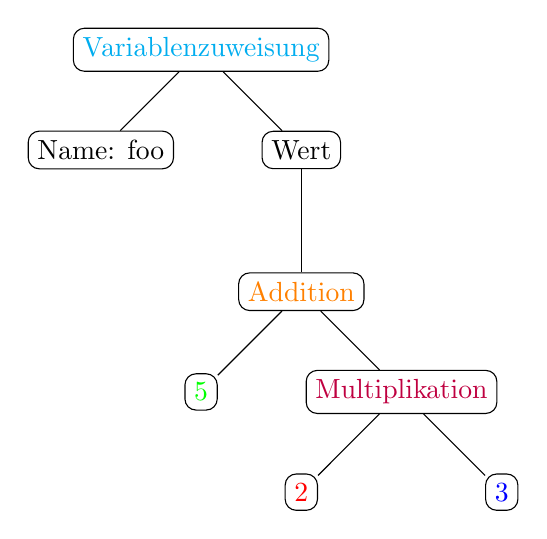
\begin{tikzpicture}[
                        node distance=1.8cm,
                        auto,
                        block/.style={
                            rectangle,
                            draw,
                            align=center,
                            rounded corners
                        },
                        line/.style={
                            draw,
                        }]

                        \node (variable_declaration) [text=cyan, block] {Variablenzuweisung};
                        \node (variable_name) [block, below left of=variable_declaration] {Name: foo};
                        \node (variable_value) [block, below right of=variable_declaration] {Wert};
                        \node (addition) [text=orange, block, below of=variable_value] {Addition};
                        \node (addition_left) [text=green, block, below left of=addition] {5};
                        \node (multiplication) [text=purple, block, below right of=addition] {Multiplikation};
                        \node (multiplication_left) [text=red, block, below left of=multiplication] {2};
                        \node (multiplication_right) [text=blue, block, below right of=multiplication] {3};

                        \draw [line] (variable_declaration) -- (variable_name);
                        \draw [line] (variable_declaration) -- (variable_value);
                        \draw [line] (variable_value) -- (addition);
                        \draw [line] (addition) -- (addition_left);
                        \draw [line] (addition) -- (multiplication);
                        \draw [line] (multiplication) -- (multiplication_left);
                        \draw [line] (multiplication) -- (multiplication_right);

                        % \draw [line, blue] (multiplication_right) 
                        %     -- ++(3.15, 0cm)
                        %     -- ++(0cm, 2.5cm)
                        %     -- ++(0.1cm, 0cm)
                        %     -- ++(0cm, 0.6cm) 
                        %     -- ++(0.1cm, 0cm) 
                        %     -- ++(-0.1cm, 0cm) 
                        %     -- ++(0cm, -1.4cm) 
                        %     -- ++(0.1cm, 0cm);

                        % \draw [line, red] (multiplication_left)  
                        %     -- ++(0cm, 0.3cm)
                        %     -- ++(5.5cm, 0cm)
                        %     -- ++(0cm, 3.2cm)
                        %     -- ++(0.3cm, 0cm)
                        %     -- ++(0cm, 1.0cm)
                        %     -- ++(0.1cm, 0cm)
                        %     -- ++(-0.1cm, 0cm)
                        %     -- ++(0cm, -1.3cm)
                        %     -- ++(0.1cm, 0cm);

                        % % 5
                        % \draw [line] (addition_left) -- ++(7.1cm, 4.2cm)
                        %     -- ++(0cm, 0.6cm)
                        %     -- ++(0.1cm, 0cm)
                        %     -- ++(-0.1cm, 0cm)
                        %     -- ++(0cm, -0.95cm)
                        %     -- ++(0.1cm, 0cm);

                        % \draw [line, green] (addition_left) 
                        % -- ++(0cm, 0.3cm)
                        % -- ++(6.6cm, 0cm)
                        % -- ++(0cm, 3.9cm)
                        % -- ++(0.45cm, 0cm)
                        % -- ++(0cm, 0.4cm)
                        % -- ++(0.1cm, 0cm)
                        % -- ++(-0.1cm, 0cm)
                        % -- ++(0cm, -1.36cm)
                        % -- ++(0.1cm, 0cm);
                        % ;

                        % \draw [line] (multiplication) -- ++(4.5cm, 0.2cm)
                        %     -- ++(0cm, 0.22cm)
                        %     -- ++(0.1cm, 0cm)
                        %     -- ++(-0.1cm, 0cm)
                        %     -- ++(0cm, -0.36cm)
                        %     -- ++(0.1cm, 0cm);

                        % \draw [line, purple] (multiplication)
                        % -- ++(4.5cm, 0cm)
                        % -- ++(0cm, 0.315cm)
                        % -- ++(0.1cm, 0cm)
                        % -- ++(-0.1cm, 0cm)
                        % -- ++(0cm, -0.36cm)
                        % -- ++(0.1cm, 0cm);




                        % % addition

                        % \draw [line] (addition) -- ++(5.78cm, -1.6cm)
                        %     -- ++(0cm, 0.22cm)
                        %     -- ++(0.1cm, 0cm)
                        %     -- ++(-0.1cm, 0cm)
                        %     -- ++(0cm, -0.36cm)
                        %     -- ++(0.1cm, 0cm);

                        % \draw [line, orange] (addition)
                        % -- ++(5.12cm, 0cm)
                        % -- ++(0, -1.6cm)
                        % -- ++(0.68cm, 0)
                        % -- ++(0, 0.22cm)
                        % -- ++(0.1cm, 0)
                        % -- ++(-0.1cm, 0)
                        % -- ++(0, -0.36cm)
                        % -- ++(0.1cm, 0);

                        % % foo
                        % \draw [line] (variable_declaration) -- ++(7.05cm, -5.5cm)
                        %     -- ++(0cm, 0.6cm) 
                        %     -- ++(0.1cm, 0cm) 
                        %     -- ++(-0.1cm, 0cm) 
                        %     -- ++(0cm, -0.85cm) 
                        %     -- ++(0.1cm, 0cm);

                        % \draw [line, cyan] (variable_declaration)
                        % -- ++(6.35cm, 0)
                        % -- ++(0, -5.5cm)
                        % -- ++(0.7cm, 0)
                        % -- ++(0, 0.6cm)
                        % -- ++(0.1cm, 0)
                        % -- ++(-0.1cm, 0)
                        % -- ++(0, -0.85cm)
                        % -- ++(0.1cm, 0);

                    \end{tikzpicture}
                \end{minipage}\hspace{3cm} &
                \begin{minipage}{0.45\textwidth}
                    \lstset{
                    moredelim=[il][\textcolor{orange}]{O},
                    moredelim=[il][\textcolor{green}]{G},
                    moredelim=[il][\textcolor{red}]{R},
                    moredelim=[il][\textcolor{blue}]{B},
                    moredelim=[il][\textcolor{cyan}]{C},
                    moredelim=[il][\textcolor{purple}]{P},
                    }
                    \begin{lstlisting}
G%_3 = alloca i64
Gstore i64 5, i64* %_3
G%_2 = load i64, i64* %_3
R%_6 = alloca i64
Rstore i64 2, i64* %_6
R%_5 = load i64, i64* %_6
B%_8 = alloca i64
Bstore i64 3, i64* %_8
B%_7 = load i64, i64* %_8
P%_9 = mul i64 %_5, %_7
O%_10 = add i64 %_2, %_9
C%_foo_0 = alloca i64
Cstore i64 %_10, i64* %_foo_0
                    \end{lstlisting}
                \end{minipage}
            \end{tabular}
        \end{center}

    Es ist zu erkennen, dass mein Compiler den Rechenausdruck zerlegt und die Operatorrangfolge beachtet.
    Jede im Ausdruck vorkommende Zahl wird in 3 Befehle übersetzt:
    \begin{itemize}
        \item \texttt{alloca i64} allokiert Speicher für die Zahl
        \item \texttt{store i64 <Zahl>, i64* \%<Variable>} schreibt die Zahl in den allokierten Speicher
        \item \texttt{load i64, i64* \%<Variable>} lädt die Zahl aus dem allokierten Speicher
    \end{itemize}

    Mein Compiler speichert die Zahl also eigentlich unnötigerweise, man könnte auch die Berechnung ohne ein Zwischenspeichern
    durchführen:
    Eine optimierte Version könnte z.B. so aussehen:
    
    \begin{lstlisting}
        %_0 = add i64 5, 0
        %_1 = add i64 2, 0
        %_2 = add i64 3, 0
        %_3 = mul i64 %_1, %_2
        %_4 = add i64 %_0, %_3
        %_foo_0 = alloca i64
        store i64 %_4, i64* %_foo_0
    \end{lstlisting}

    oder sogar noch kürzer:

    \begin{lstlisting}
        %_0 = mul i64 2, 3
        %_1 = add i64 5, %_0
        %_foo_0 = alloca i64
        store i64 %_1, i64* %_foo_0
    \end{lstlisting}

    
    Um den generierten LLVM IR Code nun in eine ausführbare Datei umzuwandeln, 
    verwendet mein Compiler eine lokale Installation des Clang Compilers (sofern vorhanden).


